\chapter{硬件模块介绍}

\section{基于FIFO的可变长移位寄存器设计}

\begin{figure}[h]
    \centering
    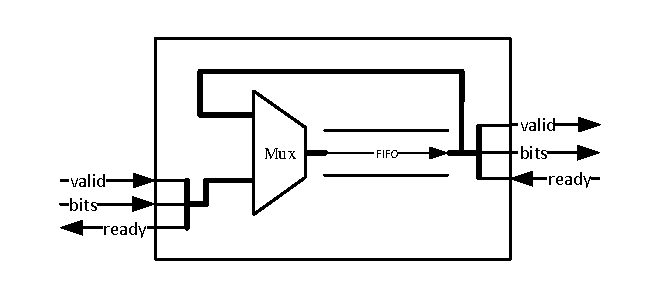
\includegraphics{../pdf/fifoshift.pdf}\\
    \caption{FIFO Shift}
\end{figure}
利用FIFO的先入先出特性,配合外部控制信号可以构造一个最大位宽为FIFO深度的移位寄存器。
首先,模块中的Mux将FIFO接口入模块输入信号连接,此时数据被写入FIFO中,当数据输入过程完成之后,Mux将模块内的FIFO输入与输出对接,
此时便形成了一个数据环路,FIFO输出的数据被输入给FIFO的输入,使数据一直保留在FIFO中。

实际使用时,FIFO深度被配置为256,位宽为16bit。第一阶段,FIFO输入通过Mux与模块的输入对接,接受来自外部的图像或者卷积核信息,第一阶段取数完成后进入第二阶段——计算,此时FIFO的输入与FIFO的输出对接,吐出的数据再次被存入FIFO中,以达到移位寄存器的功能。

需要说明的是,,该构造读数时每次只能读取最末端的数据,

    \subsection{BRAM与DRAM选择}

\section{SRAM部分在FPGA中的优化}

\section{基于Xilixn 7Series FPGA片上DSP的高性能乘法器}

\section{PE单元构造}

\section{用于数据分发的简易NoC设计}

\section{PE阵列生成器}
    \subsection{计算流程}

\section{顶层接口设计}

\section{本章小结}
% \subsection{二级节标题}

% \subsubsection{三级节标题}

% \paragraph{四级节标题}

% \subparagraph{五级节标题}

% \section{脚注}

% Lorem ipsum dolor sit amet, consectetur adipiscing elit, sed do eiusmod tempor
% incididunt ut labore et dolore magna aliqua. Ut enim ad minim veniam, quis
% nostrud exercitation ullamco laboris nisi ut aliquip ex ea commodo consequat.
% Duis aute irure dolor in reprehenderit in voluptate velit esse cillum dolore eu
% fugiat nulla pariatur. Excepteur sint occaecat cupidatat non proident, sunt in
% culpa qui officia deserunt mollit anim id est laborum.
% \footnote{This is a long long long long long long long long long long long long
% long long long long long long long long long long footnote.}
